\documentclass{homework}
\usepackage[utf8]{inputenc}
\usepackage{xspace,color,url,listings,graphicx,float,amsmath,amssymb,braket,subcaption}
\graphicspath{{./graphs/}} %location of images

\lstset{commentstyle=\color{red},keywordstyle=\color{black},
showstringspaces=false}
\lstnewenvironment{rc}[1][]{\lstset{language=R}}{}
\newcommand{\ri}[1]{\lstinline{#1}}  %% Short for 'R inline'

\lstset{language=R}             % Set R to default language

\newcommand{\hwname}{Shara Duong, Charles Colgan, Josh Borders}
\newcommand{\hwnum}{5}

\newcommand{\hwtype}{Homework}
\newcommand{\hwclass}{MATH 6350}

\begin{document}

\maketitle
Shara Duong: Wrote code.\\
Charles Colgan: Edited code and text, generated figures.\\
Josh Borders: Wrote text, edited tables and code.

\question % 1
After applying PCA to the features, we found that 104 features explained 95\% of the variance in our data. Using these features, we randomly selected 80\% of the cases in each class to be our training set and the remaining 20\% to be the testing sets. The respective sizes of the sets are displayed in Table \ref{sampling}.

\begin{table}[h]
    \centering
    {\begin{tabular}{c|ccc}
         &Training&Testing&Total\\\hline
         Bitstream&1837&459&2296\\
         Consolas&1828&457&2285\\
         Ebrima&1379&344&1723\\\hline
         Total&5044&1260
    \end{tabular}}\\
    \caption{Number of Cases for Each Class}
    \label{sampling}
\end{table}

Since the classes are approximately balanced, we did not employ cloning or under-sampling. The combination of all the training cases across the three classes resulted in a training set of size 5044, and a testing set of size 1260.

\question % 2

\textbf{1)} The Random Forest algorithm is an extension of single tree classification. The tree classifier splits a training set on those features which have the greatest discriminatory power, continuing the splitting process until each subset of cases ("leaf") is pure, with all cases being from the same class. The tree then uses the criteria it trained on to classify the testing data. However, a single tree will often classify these testing cases incorrectly due to over-fitting, resulting in impure leaves and an unreliable model.\\\\ 
The general solution to this problem is to grow a "forest" of trees, where each tree is designed differently. While each still splits on the features to reach total purity, the features available to each tree are randomized. Instead of having every available feature to split on, a random selection of features equal to the square root of the total number of features is used. Additionally, each tree is trained on a random selection of only two-thirds of the training set. This results in a classifier containing a large number of varied trees.\\\\
Cases from the training set that were not used to build a particular tree are considered to be outside the classifications made by that tree, or "out of bag". Such out of bag cases may be considered hidden, random testing sets. The out of bag cases for each tree are then processed by the tree for classification. Confusion matrices are used to determine the forest's total out of bag error rate.\\\\ 
After any necessary fine-tuning, the forest is then used on the testing set. Each case in the testing set is then sent to this classifier, and it travels each tree until the tree returns a classification. The final determination of the cases class is made by assessing the classification given by all trees, and then taking the plurality. Additional confusion matrices are then employed to determine if the cases were classified correctly, where the errors were located, and so on.

\textbf{2)} We used the randomForest() function from the randomForest package in R. Below is a sample function call, stored in the rfTrain object:
\begin{rc}
rfTrain = randomForest(font~., data=TRAINSET, ntree=100, mtry=sqrt(r))
\end{rc}
The first argument is the formula; in our case, we wanted to predict the class label (in this case font), using all of the features in our training data, TRAINSET. The number of trees we grew was 100, and the mtry parameter restricted the number of features used to build each tree at the square root of r, which was approximately 10. An additional argument, \textit{importance}, computes the numerical importance of the features, though this was not implemented in the sample. The primary ways of modifying the function are to change the number of trees and/or the number of available features.\\\\
The result of the function is stored in the rfTrain object, which has many outputs. There are pieces of information which verify the function call (e.g., one can check how many trees were grown with \textit{ntrees}, the type - classification, regression, unsupervised learning - of the function with \textit{type}, and so on), but we will focus on those metrics pertinent to our results. \begin{itemize}
    \item The \textit{confusion} command confusion matrix returns the number of training cases both successfully and unsuccessfully predicted, in addition to the error percentage for each class.
    \item The \textit{err.rate} command returns a list of every tree and its respective out of bag error rate, i.e., the proportion of out of bag cases each tree mis-classified.
    \item The \textit{importance} lists each feature's importance in reducing the impurity (the Gini) of the classification, and also the mean decrease in accuracy of the classification if the particular feature were removed from the data set.
\end{itemize}

\textbf{3)} The predict() function in R takes the Random Forest object and uses it on a new data set. Our function call is below:
\begin{rc}
rfPred = predict(rfTrain, TESTSET, type='response')
\end{rc}
The function applies the rfTrain object to the testing set, TESTSET. In other words, the testing data travels through the random forest generated by the training set. The type='response' argument tells the function to compute the predicted class values for each case, rather than a probability vector.\\\\
The output of the predict function is a list of cases and their associated predicted value.

\textbf{4)} The performance outputs of the function are the confusion matrix - which returns the percentage of cases correctly classified for each row/column pair on its diagonal - and the \textit{importance} output, which presents a list of the features' importance, measured by both the mean decrease in accuracy if the feature is excluded and the reduction in the Gini coefficient caused by the presence of the feature. 

\question % 3
\textbf{1)} We grew a random forest with 100 trees and mtry = sqrt(p) available features. Table \ref{rf100} shows the confusion matrices for both training and testing sets. This implementation of random forest has a global accuracy on the training set of \textbf{81.7\%} and \textbf{83.5\%} for the testing set. It is odd for the classifier to perform better on the testing set than the training set, and the increase in global accuracy is due almost entirely to the classifier being more accurate with Ebrima cases.

\begin{table}[H]
    \centering
    \subfloat[Training Set]{\begin{tabular}{c|ccc}
         &BITSTREAM&CONSOLAS&EBRIMA\\\hline
         BITSTREAM&0.947&0.039&0.015\\
         CONSOLAS&0.055&0.829&0.115\\
         EBRIMA&0.036&0.335&0.629\\\hline
         Global Accuracy&0.817
    \end{tabular}}\\
    \subfloat[Testing Set]{\begin{tabular}{c|ccc}
         &BITSTREAM&CONSOLAS&EBRIMA\\\hline
         BITSTREAM&0.965&0.026&0.009\\
         CONSOLAS&0.053&0.823&0.125\\
         EBRIMA&0.023&0.299&0.677\\\hline
         Global Accuracy&0.835
    \end{tabular}}
    \caption{Confusion Matrices for 100 Trees, mtry=sqrt(p)}
    \label{rf100}
\end{table}

\textbf{2)} We then implemented random forest for a wide number of trees, growing forests with one tree all the way up to forests with 400 trees. This took approximately one hour on a laptop with an Intel i7 processor, enough time for your humble author to watch an episode of The Great British Baking Show. The confusion matrices for six of these forests, ntrees = {10, 50, 100, 200, 300, 400}, are displayed in Table \ref{manyrf_1} and \ref{manyrf_2}. We observe that the global accuracy levels off at 50 trees, with fluctuations on the order of less than one percentage point as the number of trees increases to 400. This aligns well with the display of Figure \ref{classacc}, where accuracy is approximately level from 50 to 400.\\\\We are also interested in the prediction accuracy of each class, which is displayed in Figure \ref{classacc}. Across all values of trees, Bitstream is classified most accurately, while Ebrima is classified least accurately. Each class's respective accuracy begins to level off around 50 trees. We used R to calculate where global accuracy is greatest, and that number is \textbf{171 trees}.

\begin{table}[H]
    \centering
    \subfloat[10 Trees]{\begin{tabular}{c|ccc}
         &BITSTREAM&CONSOLAS&EBRIMA\\\hline
         BITSTREAM&0.943&0.039&0.017\\
         CONSOLAS&0.094&0.742&0.164\\
         EBRIMA&0.032&0.340&0.628\\\hline
         Global Accuracy&0.779
    \end{tabular}}\\
    \subfloat[50 Trees]{\begin{tabular}{c|ccc}
         &BITSTREAM&CONSOLAS&EBRIMA\\\hline
         BITSTREAM&0.961&0.022&0.017\\
         CONSOLAS&0.066&0.812&0.123\\
         EBRIMA&0.038&0.297&0.666\\\hline
         Global Accuracy&0.823
    \end{tabular}}\\
             \subfloat[100 Trees]{\begin{tabular}{c|ccc}
         &BITSTREAM&CONSOLAS&EBRIMA\\\hline
         BITSTREAM&0.959&0.031&0.011\\
         CONSOLAS&0.059&0.810&0.131\\
         EBRIMA&.029&0.323&0.648\\\hline
         Global Accuracy&0.842
    \end{tabular}}\\
    \caption{Testing Set Confusion Matrices for Different Numbers of Trees}
    \label{manyrf_1}
\end{table}

\begin{table}[H]
    \centering
    \subfloat[200 Trees]{\begin{tabular}{c|ccc}
         &BITSTREAM&CONSOLAS&EBRIMA\\\hline
         BITSTREAM&0.965&0.024&0.011\\
         CONSOLAS&0.053&0.842&0.105\\
         EBRIMA&0.029&0.291&0.680\\\hline
         Global Accuracy&0.838
    \end{tabular}}\\
        \subfloat[300 Trees]{\begin{tabular}{c|ccc}
         &BITSTREAM&CONSOLAS&EBRIMA\\\hline
         BITSTREAM&0.963&0.024&0.013\\
         CONSOLAS&0.055&0.838&0.107\\
         EBRIMA&0.029&0.288&0.683\\\hline
         Global Accuracy&0.842
    \end{tabular}}\\
    \subfloat[400 Trees]{\begin{tabular}{c|ccc}
         &BITSTREAM&CONSOLAS&EBRIMA\\\hline
         BITSTREAM&0.965&0.022&0.013\\
         CONSOLAS&0.057&0.832&0.112\\
         EBRIMA&0.029&0.285&0.686\\\hline
         Global Accuracy&0.843
    \end{tabular}}
    \caption{Testing Set Confusion Matrices for Different Numbers of Trees cont.}
    \label{manyrf_2}
\end{table}

\begin{figure}[H]
    \centering
    \subfloat[Total]{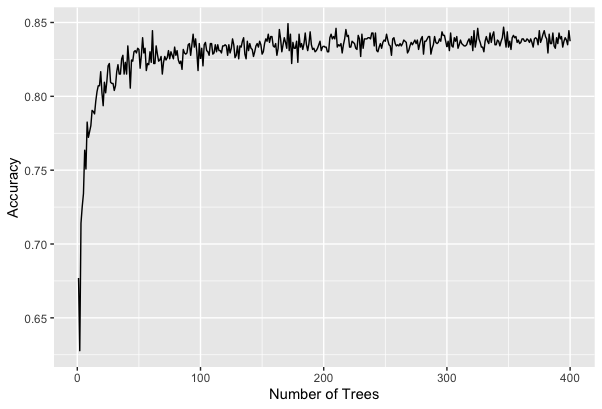
\includegraphics[width=9cm,height=6cm]{images/ACC_TOT.png}} 
    \subfloat[By Class]{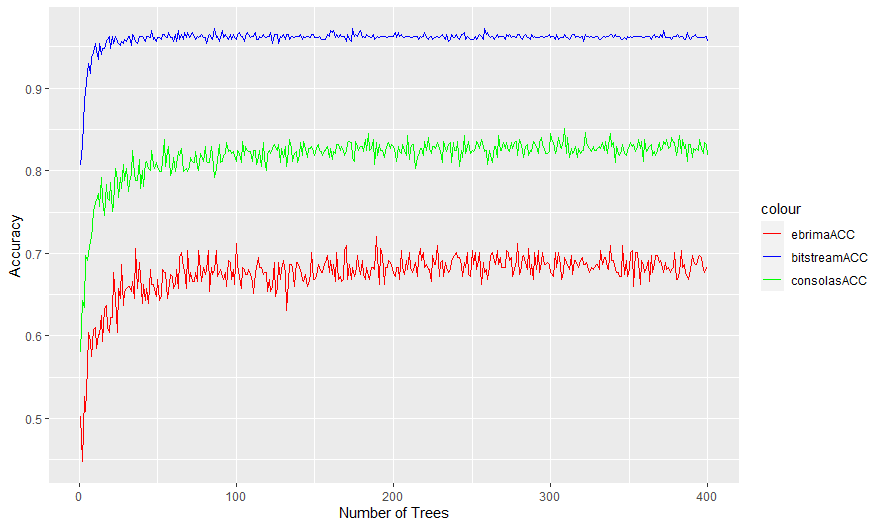
\includegraphics[width=9cm,height=6cm]{images/ACC_CLS.png}} 
    \caption{Classification Accuracy}
    \label{classacc}
\end{figure}

\question % 4
\textbf{1)} With 171 selected to be our best number of trees, we once again applied the Random Forest function with ntree=171 and ntry = sqrt(p). The importance of the features was computed in the Random Forest object, and the eigenvalues associated with these features was also computed. A scatter plot is displayed in Figure \ref{scatter}, indicating that the smaller eigenvalues have greater importance to the classifier.

\begin{figure}[H]
    \centering
    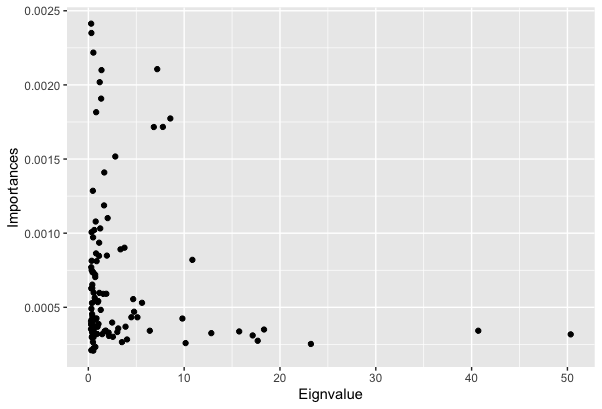
\includegraphics[width=13cm]{images/IMP.png}
    \caption{Eigenvalues vs. Importance Scatter Plot}
    \label{scatter}
\end{figure}

\textbf{2)} We then selected new training and testing sets, using the same methods described in Question 1 (i.e., randomly select 80\% of the cases in each class for training, the remaining 20\% for testing). We applied random forest with 171 trees and ntry = sqrt(p), seeing if our results are robust to the selection of different training and testing sets.\\\\ 
We used the random forest classifier trained on the new training set to predict the classes for the testing set's cases. The confusion matrices for the testing sets of both the old and new classifiers are shown in Table \ref{newconfusion}. The new random forest has a global accuracy of approximately 82.9\%, while the old's is 82.3\%\\\\ 
We computed 90\% confidence intervals for each random forest implementation's global accuracy, allowing us to further compare the performance of these two different random forests, each with 171 trees. The formula used for the confidence interval was that for a population proportion, \begin{math} a \pm Z_{alpha/2} * \sqrt{(a)*(1-a)/n}\end{math}, where \textit{a} is the global accuracy estimate. The 90\% confidence interval for the old random forest's global accuracy is (0.811,0.846), while the 90\% CI for the new random forest's global accuracy is (0.806,0.842). There is substantial overlap between the two confidence intervals, indicating that a forest of 171 trees for this application is robust to the selection of different training and testing sets.

\begin{table}[H]
    \centering
        \subfloat[Old Testing Set]{\begin{tabular}{c|ccc}
         &BITSTREAM&CONSOLAS&EBRIMA\\\hline
         BITSTREAM&0.961&0.0267&0.013\\
         CONSOLAS&0.066&0.822&0.112\\
         EBRIMA&0.029&0.285&0.686\\\hline
         Global Accuracy&0.823
    \end{tabular}}\\
    \subfloat[New Testing Set]{\begin{tabular}{c|ccc}
         &BITSTREAM&CONSOLAS&EBRIMA\\\hline
         BITSTREAM&0.950&0.035&0.015\\
         CONSOLAS&0.070&0.834&0.096\\
         EBRIMA&0.055&0.285&0.6560\\\hline
         Global Accuracy&0.829
    \end{tabular}}
    \caption{Confusion Matrices for Different Testing Sets with 171 Tree Random Forest}
    \label{newconfusion}
\end{table}

\question % 5
\textbf{1)} We now implement random forest three separate times, focusing on the ability of random forest to predict a single class correctly. For example, our first random forest implementation will try to predict Bitstream correctly, while treating the fonts Consolas and Ebrima as being of the same class. Since our original classes were approximately balanced, this requires us to clone the cases of Bitstream one time, giving us 3674 cases of class Bitstream and 3207 cases of class Consolas/Ebrima for our training set. This leaves 918 cases of class Bitstream and 801 cases of class Consolas/Ebrima for our testing set. Similar procedures are followed for our second and third random forests, focusing on Consolas and Ebrima, respectively.\\\\ The confusion matrices are displayed in Table \ref{segforests}. The first random forest comparing Bitstream vs the other fonts performs the best, with a global accuracy of 96.6\%. This indicates that random forest identifies most Bitstream cases quite easily. The third matrix listed performs the worst, as random forest has comparative difficulty recognizing Ebrima cases, hitting on only 65.4\% of Ebrima observations. While this is roughly the same performance on Ebrima cases as the three-class classifier, it is especially disappointing that random forest could not determine the simpler answer of whether a case was of class Ebrima or not. In sum, random forest seems to confuse Ebrima and Consolas cases, while recognizing Bitstream cases with high accuracy.

\begin{table}[H]
    \centering
    \subfloat[Bitstream vs. Others]{\begin{tabular}{c|ccc}
         &BITSTREAM&CONSOLAS/EBRIMA\\\hline
         BITSTREAM&0.961&0.039\\
         CONSOLAS/EBRIMA&0.027&0.973\\\hline
         Global Accuracy&0.966
    \end{tabular}}\\
        \subfloat[Consolas vs. Others]{\begin{tabular}{c|ccc}
         &CONSOLAS&BITSTREAM/EBRIMA\\\hline
         CONSOLAS&0.733&0.115\\
         BITSTREAM/EBRIMA&0.267&0.885\\\hline
         Global Accuracy&0.804
    \end{tabular}}\\
        \subfloat[Ebrima vs. Others]{\begin{tabular}{c|ccc}
         &EBRIMA&BITSTREAM/CONSOLAS\\\hline
         EBRIMA&0.654&0.078\\
         BITSTREAM/CONSOLAS&0.346&0.922\\\hline
         Global Accuracy&0.810
    \end{tabular}}
    \caption{Confusion Matrices for Two-Class Testing Sets with 171 Tree Random Forest}
    \label{segforests}
\end{table}

\textbf{2)} We now apply predictions to the same problem - identifying the cases belonging to a single class - using the random forest classifier from section 4.1 to predict the class of cases from our 5.1 testing sets. The confusion matrices are listed in Table \ref{comparison}.

\begin{table}[H]
    \centering
    \subfloat[Bitstream vs. Others]{\begin{tabular}{c|ccc}
         &BITSTREAM&CONSOLAS/EBRIMA\\\hline
         BITSTREAM&0.965&0.035\\
         CONSOLAS/EBRIMA&0.049&0.951\\\hline
         Global Accuracy&0.959
    \end{tabular}}\\
        \subfloat[Consolas vs. Others]{\begin{tabular}{c|ccc}
         &CONSOLAS&BITSTREAM/EBRIMA\\\hline
         CONSOLAS&0.812&0.188\\
         BITSTREAM/EBRIMA&0.136&0.864\\\hline
         Global Accuracy&0.836
    \end{tabular}}\\
        \subfloat[Ebrima vs. Others]{\begin{tabular}{c|ccc}
         &EBRIMA&BITSTREAM/CONSOLAS\\\hline
         EBRIMA&0.683&0.317\\
         BITSTREAM/CONSOLAS&0.068&0.932\\\hline
         Global Accuracy&0.825
    \end{tabular}}
    \caption{Confusion Matrices for Two-Class Testing Sets with Sec 4.1 Random Forest}
    \label{comparison}
\end{table}

Applying 4.1's random forest classifier to the two-class testing sets yields similar results. The change in global accuracy is less than 5\% in for all fonts and the values of the confusion matrices are also similar. Looking at the fonts individually, BITSTREAM's classification accuracy stayed around the same while CONSOLAS had the largest increase of 7.9\%. The classification of EBRIMA cases gained aroung 3\% accuracy but is still the lowest overall at 68.3\%. This suggests that the font is less distinguishable than the other two, even when predicted by a more sophisticated, three-class random forest.

\newpage
\lstinputlisting{code.R}
\end{document}